\section{Deep Learning 2}\label{deep-learning-2}

\subsection{Artificial Neural Network}\label{artificial-neural-network}

\subsubsection{Biological Neuron}\label{biological-neuron}

\begin{enumerate}
\def\labelenumi{\arabic{enumi}.}
\tightlist
\item
  神经元接收许多上游神经元的突触输入：

  \begin{itemize}
  \tightlist
  \item
    兴奋性输入产生 EPSP（Excitatory Post-Synaptic
    Potential），使膜电位上升；
  \item
    抑制性输入产生 IPSP（Inhibitory Post-Synaptic
    Potential），使膜电位下降；
  \end{itemize}
\item
  神经元对这些输入进行时间积分（temporal integration）；
\item
  当膜电位在轴丘（axon hillock / initial
  segment）处超过阈值时，神经元触发动作电位（spike）；
\item
  动作电位沿轴突传播，传递给下游神经元。
\end{enumerate}

本质上，神经元是一种\textbf{时序}的阈值非线性单元，包含输入合成、阈值触发和事件传播。

\subsubsection{SNN vs ANN}\label{snn-vs-ann}

脉冲神经网络（\textbf{Spiking Neural
Network}）与传统人工神经网络（\textbf{Artificial Neural Network}）。

特征 \textbar{} \textbf{ANN} \textbar{} \textbf{SNN} \textbar{}\\
:--- \textbar{} :--- \textbar{} :--- \textbar{}\\
Representation \textbar{} \textbf{连续激活值}（continuous
activations），每个神经元在一次前向计算中输出一个实数值 \textbar{}
以事件/\textbf{脉冲}（spikes）表示信息，信息由脉冲的时序或频率编码
\textbar{}\\
Temporal handling \textbar{}
无显式时间状态（frame-based），通常把时间维度外推或用循环结构处理
\textbar{} 显式时间动力学（temporal dynamics），需要对膜电位进行 time
integration \textbar{}\\
Computation mode \textbar{}
同步、逐层前向计算（每层一次），适合批处理与矩阵运算加速 \textbar{}
\textbf{事件驱动}（event-driven），只有在有脉冲时才发生计算，适合稀疏异步计算
\textbar{}\\
Training / Optimization \textbar{} 方便使用 backpropagation
和梯度下降算法，工具链成熟 \textbar{}
直接训练困难（梯度不连续），常用近似/替代方法（如 \textbf{surrogate
gradient}）；训练和调参更复杂 \textbar{}\\
Typical applications \textbar{}
图像、语音、自然语言等多数传统深度学习任务，端到端训练容易实现
\textbar{}
适合低功耗、在线、实时与时序敏感任务；在类脑（\textbf{neuromorphic}）硬件上有优势
\textbar{}\\
Biological plausibility vs engineering \textbar{}
工程友好但生物意义较弱，与真实神经元差异大 \textbar{}
更接近生物神经元的放电机制，但为工程实用性牺牲了训练易用性 \textbar{}

\textbf{注}：

\begin{itemize}
\tightlist
\item
  脉冲发放是二值、非连续的事件，梯度不存在或为零。通常使用\textbf{surrogate
  gradient}（替代梯度）方法将脉冲函数近似为可导函数。也可以先在 ANN
  上训练再转换为 SNN（ANN-to-SNN conversion）。
\item
  当系统对延迟、能耗、异步事件处理有严格要求时（例如传感器事件流、嵌入式/边缘设备、神经形态芯片等），SNN
  的事件驱动特性和稀疏计算可能带来明显优势。
\end{itemize}

\begin{center}\rule{0.5\linewidth}{0.5pt}\end{center}

\subsection{CNN}\label{cnn}

卷积神经网络（Convolutional Neural Network）。

\subsubsection{Convolutional Layer}\label{convolutional-layer}

\begin{itemize}
\tightlist
\item
  输入尺寸：\(W_{in} \times H_{in} \times C\)
\item
  filter 尺寸：\(F \times F \times C\)
\item
  filter 个数：\(K\)
\item
  stride 步长：\(S\)
\item
  padding 填充：\(P\)
\item
  输出尺寸：\(W_{out} \times H_{out} \times K\) 其中 \[
    \begin{aligned}
    W_{out} = \left\lfloor\frac{W_{in} - F + 2P}{S}\right\rfloor + 1 \\
    H_{out} = \left\lfloor\frac{H_{in} - F + 2P}{S}\right\rfloor + 1
    \end{aligned}
    \]
\item
  参数数量： \[
    \text{Conv Params} = (F \times F \times C + 1) \times K
    \] 每个 filter 有 \(F \times F \times C\) 个可训练权重以及一个
  bias。
\end{itemize}

\textbf{注}：filter 深度等于通道数，故每个位置不再是乘积，而应该是点积。

\subsubsection{Padding}\label{padding}

\textbf{Padding Size}：

\begin{itemize}
\tightlist
\item
  Valid：\(P = 0\)
\item
  Same Padding： \[
    P = \left\lfloor\frac{F-1}{2}\right\rfloor
    \]
\item
  Full Padding： \[
    P = F - 1
    \] 确保每个输入元素被卷积次数相同。
\end{itemize}

\textbf{Padding Content}：

\begin{itemize}
\tightlist
\item
  Zero Padding：填充 \(0\)
\item
  Constant Padding：填充固定常数 \(c\)，常用均值
\item
  Reflect Padding：镜像反射边缘
\item
  Replicate Padding：复制边缘
\item
  Circular Padding：循环填充
\end{itemize}

\subsubsection{Pooling}\label{pooling}

池化（Pooling）是通过下采样（spatial
downsampling），减小特征图尺寸，提取更抽象、更不变的表示。

\textbf{Pooling Type}：

\begin{itemize}
\tightlist
\item
  Average pooling；常用
\item
  Max pooling；最常用
\item
  Sum pooling：较少
\end{itemize}

\textbf{注}：

\begin{itemize}
\tightlist
\item
  池化操作没有可训练参数，输出尺寸公式与 Conv Layer 完全相同。
\item
  池化可以增加对微小\textbf{平移}和微小\textbf{旋转}的\textbf{不变性}（invariance）。
\item
  不一定需要池化，通过选定步长也可以替代池化的作用。
\end{itemize}

\subsubsection{Conv Layer vs FC Layer}\label{conv-layer-vs-fc-layer}

\begin{itemize}
\tightlist
\item
  \textbf{Parameter Count}： 参考
  convolutional-layer 中的定义，考虑
  bias 时两者的参数数量分别为：
  \[
    \begin{aligned}
    \text{Conv Params} &= (F \times F \times C + 1) \times K \\
    \text{FC Params} &= (W_{\text{in}} \times H_{\text{in}} \times C + 1) \times (W_{\text{out}} \times H_{\text{out}} \times K)
    \end{aligned}
  \]
  显然 Convolution 少了不只一点。
\item
  \textbf{Sparse Connectivity}： Conv
  只进行\textbf{稀疏连接}，也即每个像素点只与它相邻的点进行连接；而 FC
  是全连接的。所以 Conv 之后仍保留了\textbf{空间位置信息}。

  \centering
  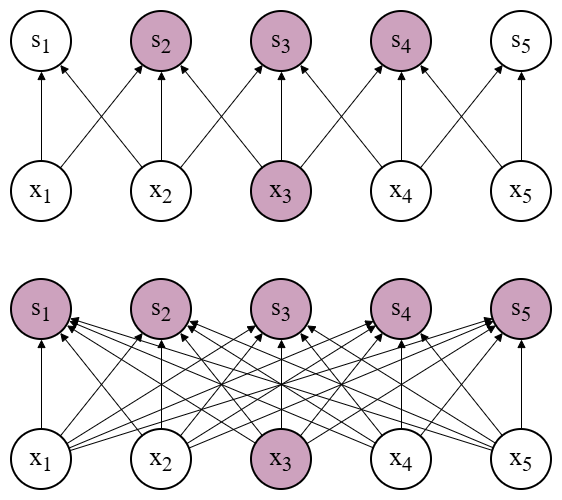
\includegraphics[width=\linewidth]{assets/05-deep-learning-2-01-sparse-connectivity.png}
  \captionof{figure}{图 1：稀疏连接}
\item
  \textbf{Parameter Sharing}： Conv
  进行\textbf{参数共享}，也即同一卷积核在整张图像上复用；而 FC
  则是各边权互不相同。这种参数共享使得 Conv
  天然具有（微小）\textbf{平移等变性}。

  \centering
  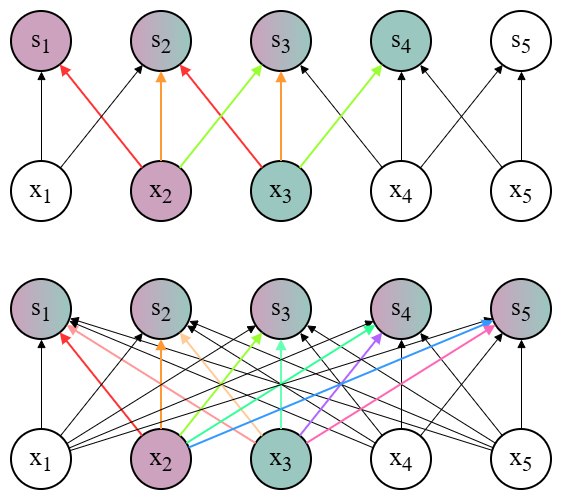
\includegraphics[width=\linewidth]{assets/05-deep-learning-2-02-parameter-sharing.drawio.png}
  \captionof{figure}{图 2：参数共享，颜色相同的边参数相等}
\end{itemize}

本质上，MLP 是 CNN 的超集。若用 \(\mathcal{F}_{\text{CNN}}\) 和
\(\mathcal{F}_{\text{MLP}}\) 分别表示 CNN 与 MLP
能够学习的函数集合，则： \[
\mathcal{F}_{\text{MLP}} \supseteq \mathcal{F}_{\text{CNN}}
\]

所以 MLP 其实更加 \textbf{expressive}。

但是实际训练时，我们很难在 MLP
如此广阔的参数空间中，优化寻找到满足所需性质（比如平移等变性）的那种解。
所以我们不妨在 MLP
的一个\textbf{特殊的}、\textbf{满足一定性质}（比如平移等变性）的子集中进行寻找，比如在
CNN 中寻找。

这就是利用 \textbf{Inductive Bias}（归纳偏见）简化问题。

\begin{center}\rule{0.5\linewidth}{0.5pt}\end{center}

\subsection{Training a CNN}\label{training-a-cnn}

\subsubsection{Pipeline}\label{pipeline}

\begin{enumerate}
\def\labelenumi{\arabic{enumi}.}
\tightlist
\item
  Data preparation and preprocessing
\item
  Weight initialization
\item
  Set a loss function
\item
  Start optimization
\end{enumerate}

\subsubsection{Data Preprocessing}\label{data-preprocessing}

为加速训练收敛、减少过拟合、提升鲁棒性，我们需要对数据进行预处理。

\begin{itemize}
\item
  \textbf{Normalization}：

  \begin{itemize}
  \item
    减均值（zero-mean）、除方差（unit variance）。注意对于 RGB
    图像，需要对每个通道分别进行操作（per-channel mean）。
  \item
    直接将像素值缩放到 \([0,1]\)。

    这样可以使得数值更稳定，并且避免只向一个方向优化。
  \end{itemize}
\item
  \textbf{Augmentation}：随机裁剪、翻转、旋转、颜色扰动、缩放、平移、弹性变形等，以增强泛化能力。
\item
  \textbf{Batching and Shuffle}：随机打乱并按 mini-batch 用于训练。
\item
  \textbf{Dataset Split}：划分训练集、验证集、测试集。
\end{itemize}

\textbf{注}：验证集通常不做随机增强（或只做确定性变换），以确保评估一致性。训练集可做随机增强。

\subsubsection{Weight Initialization}\label{weight-initialization}

梯度初始化很重要：

\begin{itemize}
\tightlist
\item
  初始化太小，信号逐层衰减，\textbf{梯度消失}，网络无法训练；
\item
  初始化太大，信号逐层放大，\textbf{梯度爆炸}，数值不稳定；
\end{itemize}

所以我们需要合理初始化权重。下面先给出权重初始化的核心考虑因素，也即权重分布的方差。

\textbf{引理}：

对于神经网络的某一层，记：

\begin{itemize}
\tightlist
\item
  $\text{fan}_{\text{in}}$ 为该层输入单元数量，例如 Conv 时为
  $F \times F \times C$
\item
  $\text{fan}_{\text{out}}$ 为该层输出单元数量，例如 Conv 时为
  $F \times F \times K$
\end{itemize}

假设：

\begin{enumerate}
\def\labelenumi{\arabic{enumi}.}
\tightlist
\item
  输入 $x_i$ 独立同分布，均值 $E[x_i] = 0$，方差
  $\text{Var}(x_i) = \sigma_x^2$
\item
  权重 $w_i$ 独立同分布，均值 $E[w_i] = 0$，方差
  $\text{Var}(w_i) = \sigma_w^2$
\item
  $x_i$ 与 $w_i$ 相互独立
\item
  神经元计算为 $y = \sum_{i=1}^{n} w_i x_i$，也即忽略激活函数
\end{enumerate}

则为保持输出方差等于输入方差 $\sigma_y^2 = \sigma_x^2$，应取：
\[
\sigma_w^2 = \frac{1}{\text{fan}_{\text{in}}}
\]

\textbf{证明}：

\[
\begin{aligned}
\text{Var}(y)
&= \text{Var}\left(\sum_{i=1}^{\text{fan}_{\text{in}}} w_i x_i\right) \\
&= \sum_{i=1}^{\text{fan}_{\text{in}}} \text{Var}(w_i x_i) \\
&= \sum_{i=1}^{\text{fan}_{\text{in}}} \left( E[w_i^2] E[x_i^2] - (E[w_i]E[x_i])^2 \right) \\
&= \text{fan}_{\text{in}} \cdot \sigma_w^2 \cdot \sigma_x^2
\end{aligned}
\]

从而由 $\sigma_y^2 = \sigma_x^2$ 得：
\[
\sigma_w^2 = \frac{1}{\text{fan}_{\text{in}}}
\]

\textbf{注}：

\begin{itemize}
\tightlist
\item
  有时为了正向传播和反向传播开始时都能尽量保持方差，会取两者均值初始化，也即：
  \[
    \sigma_w^2 = \frac{1}{\text{fan}_{\text{in}} + \text{fan}_{\text{out}}}
  \]
  但下面均不考虑反向传播。要考虑只需用
  $\text{fan}_{\text{in}} + \text{fan}_{\text{out}}$ 替换 $\text{fan}_{\text{in}}$ 即可。
\item
  考虑激活函数的影响：

  当使用 \textbf{ReLU}
  激活函数时，由于负半轴置零，输出方差近似减半，需修正为： \[
    \sigma_w^2 = \frac{2}{\text{fan}_\text{in}}
    \] 当使用 \textbf{Leaky ReLU} 激活函数时，再依负半轴斜率 $
  \alpha $ 修正为： \[
    \sigma_w^2 = \frac{2}{\text{fan}_\text{in} \cdot (1+\alpha^2)}
    \] 当使用 \textbf{tanh} 激活函数时，由于在 0 附近有
  \(\tanh(z) \approx z\)，从而我们不需要修正。也即仍为： \[
    \sigma_w^2 = \frac{1}{\text{fan}_\text{in}}
    \] 不过事实上，由于
  \(\tanh(z) < z\)，所以不修正下方差会逐层缓慢减小。

  当使用 \textbf{Sigmoid} 激活函数时，由于 \(\sigma(0) = 0.5\) 且
  \(\sigma'(0) = 0.25\)， 在 0 附近有
  \(\sigma(z) \approx 0.5 + 0.25z\)，输出方差被压缩为原来的
  \(\frac{1}{16}\)，从而我们需要将权重方差放大 16 倍来补偿，修正为： \[
    \sigma_w^2 = \frac{16}{\text{fan}_\text{in}}
    \] 不过事实上，由于 sigmoid 输出均值不为
  0，且过大的初始化易使神经元进入饱和区导致梯度消失，实际使用中常采用较保守的初始化（如
  \(2/\text{fan}_\text{in}\)），或优先考虑其他激活函数。
\item
  以上策略仅保证\textbf{训练开始时}信号方差稳定，实际训练中方差必然会随参数更新而改变。
\end{itemize}

\textbf{具体初始化}：

所有初始化都可以统一为：

\begin{itemize}
\tightlist
\item
  高斯分布： \[
    W \sim \mathcal{N}(0,\ \sigma_w^2)
    \]
\item
  均匀分布： \[
    W \sim \mathcal{U}\left(-\sqrt{3\sigma_w^2},\ \sqrt{3\sigma_w^2}\right)
    \]
\end{itemize}

具体来说，

\begin{itemize}
\tightlist
\item
  对于对称激活函数（如 tanh），我们不需要修正方差，则称为
  \textbf{Xavier/Glorot 初始化}；
\item
  对于不对称激活函数（如 ReLU / Leaky
  ReLU），我们需要针对激活函数进行一些修正，则称为 \textbf{He 初始化}。
\end{itemize}

\textbf{注}：

\begin{itemize}
\tightlist
\item
  初始化仍是研究中的活跃领域（如针对
  Transformer、稀疏网络等有特殊初始化策略）。
\item
  深层网络训练还依赖 BatchNorm、ResNet 等技巧缓解梯度问题。
\end{itemize}

\subsubsection{Optimizer}\label{optimizer}

记梯度 \(g_t = \nabla_\theta \mathcal{L}(\theta_t)\)

\begin{itemize}
\item
  \textbf{SGD}： 随机梯度更新（Stochastic Gradient Descent）。 \[
    \theta_{t+1} \leftarrow \theta_t - \alpha g_t
    \] 问题在于原始 SGD 噪声大、收敛慢。
\item
  \textbf{Momentum}： \[
    v_t \leftarrow \rho v_{t-1} + (1 - \rho) g_t,\quad
    \theta_{t+1} \leftarrow \theta_t - \alpha v_t
    \] 展开即得： \[
    v_t = (1 - \rho) \sum_{i = 0}^t \rho^{t-i} g_i
    \] 其中 \(\rho\) 是动量系数/摩擦系数，常取 \(\rho = 0.9\)。\(v_t\)
  是速度，\(\theta_t\) 是位置。

  速度累积自历史梯度，有助于穿越鞍点与加速曲面方向。
\item
  \textbf{RMSProp}： \[
    s_t \leftarrow \rho s_{t-1} + (1-\rho)g_t^2,\quad
    \theta_{t+1} \leftarrow \theta_t - \alpha \frac{g_t}{\sqrt{s_t} + \epsilon}
    \] 其中 \(s_t\) 为梯度平方的移动平均。\(\epsilon = \text{1e-8}\)
  防止除零。
\item
  \textbf{Adam}： \[
    \begin{aligned}
    m_t &= \beta_1 m_{t-1} + (1-\beta_1) g_t \\
    v_t &= \beta_2 v_{t-1} + (1-\beta_2) g_t^2 \\
    \hat m_t &= \frac{m_t}{1-\beta_1^t},\quad \hat v_t = \frac{v_t}{1-\beta_2^t} \\
    \theta_{t+1} &= \theta_t - \alpha \frac{\hat m_t}{\sqrt{\hat v_t} + \epsilon}
    \end{aligned}
    \] 其中 \(m_t\) 为一阶矩，\(v_t\) 为二阶矩，\(\beta1,\ \beta_2\)
  为超参数，常取
  \(\beta_1 = 0.9,\ \beta_2 = 0.999\)。\(\epsilon = \text{1e-8}\)
  防止除零。

  本质上是在自适应学习率，一般收敛快、对超参不敏感，适合初学者作为默认选择。
\end{itemize}

\textbf{注}： Adam 一般收敛快，但是 SGD + Momentum
能够训练出更好的模型。

\subsubsection{Learning Rate}\label{learning-rate}

学习率对训练至关重要：

\begin{itemize}
\tightlist
\item
  学习率太小，收敛慢或容易陷入局部最小（undershoot）；
\item
  学习率太大，发散或在最优附近震荡（overshoot）。
\end{itemize}

建议的初始学习率约为
\([\text{1e-6}, \text{1e-3}]\)。以下是常见的学习率调度策略。

\textbf{Schedules}：

\begin{itemize}
\tightlist
\item
  \textbf{Decay Strategy}： 记 \(T\) 为总 epoch 数。

  \begin{itemize}
  \tightlist
  \item
    Fixed：\(\alpha_t = \alpha_0\)
  \item
    Step decay：每隔若干 epoch 乘以衰减因子
  \item
    Exponential：\(\alpha_t = \alpha_0 \cdot \gamma^t\)
  \item
    Linear：\(\alpha_t = \alpha_0 (1 - t/T)\)
  \item
    Cosine：\(\alpha_t = \frac{1}{2} \alpha_0 (1 + \cos(t\pi/T))\)
  \item
    Inverse sqrt：$ \alpha_t = \alpha_0 / \sqrt{t}$
  \item
    ReduceLROnPlateau：自适应策略，根据验证集表现自动调整 LR
  \end{itemize}
\item
  \textbf{Warmup
  Strategy}：训练初期学习率线性增大，再进入正常调度。解决训练初期大 LR
  导致不稳定的问题，尤其在大 batch 或 Transformer 等结构中常用。
\item
  \textbf{Stopping Strategy}：在验证集上连续若干 epoch
  无提升则停止训练。可以防止过拟合。
\end{itemize}

\textbf{注}：推荐使用 Adam 与 Fixed decay 先找到收敛的 epoch
总数，然后再使用 SGD + Momentum 与 Cosine decay 进一步训练。

\subsubsection{Iteration vs Epoch}\label{iteration-vs-epoch}

\textbf{迭代概念}：

\begin{itemize}
\tightlist
\item
  Batch size：一次 iteration 中的样本数。
\item
  Iteration：对一个 batch 的一次 propagation 与 backpropagation。
\item
  Epoch：完整遍历一次训练集，包含若干 iterations。
\end{itemize}

事实上我们有关系： \[
\text{Iterations per Epoch} \propto \frac{\text{Total Samples}}{\text{Batch Size}}
\] 我们通常在一个 Epoch 后进行可视化点采样、模型测试和参数存储。
我们调整上述量时，应考虑模型优化量。定义： \[
\begin{aligned}
\text{Total Update Magnitude}
&\propto (\text{Iterations per Epoch} \times \text{Epoch}) \times \text{Learning Rate} \\
&\propto \frac{\text{Total Samples} \times \text{Epoch} \times \text{Learning Rate}}{\text{Batch Size}}
\end{aligned}
\] 从而可见控制模型优化相同，则：

\begin{itemize}
\tightlist
\item
  若 Batch Size 和 Learning Rate 不变，增大样本数，可以减小 Epoch
\item
  若 Epoch 和样本数不变，增大 Batch Size，可以增大 Learning Rate
\end{itemize}
